\documentclass{article}

\usepackage{listings}
\usepackage{ctex}
\usepackage{amsmath}
\usepackage{graphicx}
\usepackage{epstopdf}
\usepackage{ctex}
\usepackage{cite}

\title{Mandelbrot Set 的生成与探索}
\author{罗俊勋}

\begin{document}
    \maketitle
    %这里是摘要
    \begin{abstract}
        简要回顾Mandelbrot Set的历史.展示可视化数学的美,并使用Python实现set可视化

    \end{abstract}

    %这里是引言

    \paragraph{1.引言:}

    曼德勃罗特集是一个几何图形,曾被称为“上帝的指纹”。这个点集均出自公式$:Zn+1=(Zn)^2+C$,对于非线性迭代公式$Zn+1=(Zn)^2+C,$所有
使得无限迭代后的结果能保持有限数值的复数z的集合\(也称该迭代函数的$Julia$集\)连通的$c$,构成曼德勃罗集,它是曼德勃罗教授在二十世纪七十年代发现的.
\cite{Mandelbrot-Set-Introduction}

    \paragraph{2.背景介绍:}

    Mandelbrot图形是由美国数学家曼徳勃罗教授于1975年夏天一个夜晚,在冥思苦想之余翻看儿子的拉丁文字典时想到的,起拉丁文的原意是“产生无规则的碎片”。曼德勃罗教授称此为"魔鬼的聚合物"。为此,曼德勃罗在1988年获得了"科学行为艺术大奖".

    \paragraph{3.数学理论:}

    显示曼德勃罗特集是处理位映射图像的一个例子.首先要对图像进行计算,且计算量很
大.曼德勃罗特集是复数平面中的点集,当对一个函数迭代计算时,这些点将处于准稳定状
态(quasi-stable),即将会增加或减少,但不会超过某一限度.通常该函数为:
$z_{k+1} = z_{k}^2+c$式中$z_{k+1}$是复数$z = a + bi$的第$k+1$次迭代,$c$是确定该点在复平面中位置的复数值.$z$的初始
值为$0$.迭代将一直进行下去,直到$z$的幅值大于2或者迭代次数已经达到某种任意的规定的限度.

    \paragraph{4.算法:}\par
   
    \verb|#生成网格矩阵|\par 
    \verb|X = arange(-2, .9, .002)| \& \verb|Y = arange(-1,  1, .002)|\par 
    \verb|Z = zeros((len(Y), len(X)))| Z便是一个元都是0的矩阵\par 
    
    \verb|#构造迭代函数|\par
    $ f(x):\quad  z = 0 \quad for \quad n \quad in \quad range(100):\quad z=z^2+c \quad if \quad |z| > 2:\\
     $返回n并退出循环,否则返回NaN\par 
    
    \verb|#对网格中每个点进行|$f$运算,将最后得到的矩阵Z用Imshow热图呈现
    
    最终使用的Python代码为:\par
    \begin{lstlisting}[language=Python, caption=Python example]
        # 导入库
        from pylab import *
        from numpy import NaN
        # 传入迭代上限次数
        N = int(input())
        # 定义迭代函数
        def m(a):
            z = 0
            global N #全局变量申明
            for n in range(1, N+1):
                z = z**2 + a
                if abs(z) > 2:
                    return n
            return NaN
        # 构造空矩阵
        X = arange(-2, .9, .002)
        Y = arange(-1,  1, .002)
        Z = zeros((len(Y), len(X)))
        # 填充矩阵
        for iy, y in enumerate(Y):

            for ix, x in enumerate(X):
                Z[iy,ix] = m(x + 1j * y)
        # 可视化
        imshow(Z, cmap = plt.cm.prism, interpolation = 'none',
         extent = (X.min(), X.max(), Y.min(), Y.max()))
        xlabel("Mandelbrot Set")
        ylabel("maked by luojunxun")
        savefig("wfrgure_1.esp")
        show()
        #imshow的常用参数camp改变格式,extent改变绘图区域
        \end{lstlisting}
        
    
    \paragraph{5.数值算例:}调整N和imshow的参数\par
    1.N=100,cmap=plt.cm.prism,extent=(X.min(), X.max(), Y.min(), Y.max())\par 
    \begin{figure}[h]
        \centering
        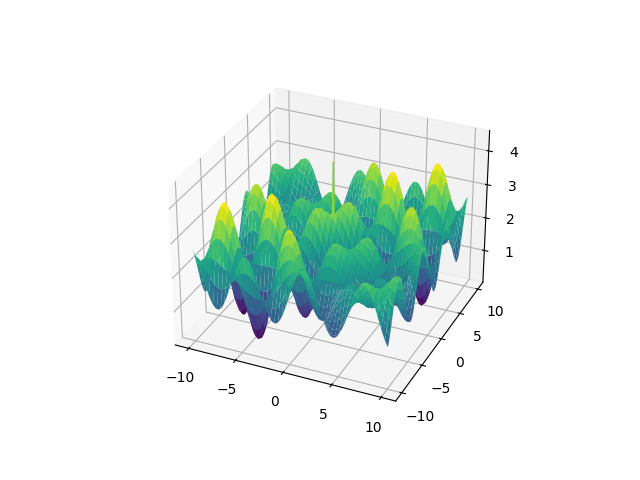
\includegraphics[scale = 0.5]{Figure_1.eps}
        \label{figure_1}
    \end{figure}
    \par \par \par 

    2.N=150,cmap=plt.cm.Blues,extent=(X.min(), X.max(), Y.min(), Y.max())\par 
    \begin{figure}[h]
        \centering
        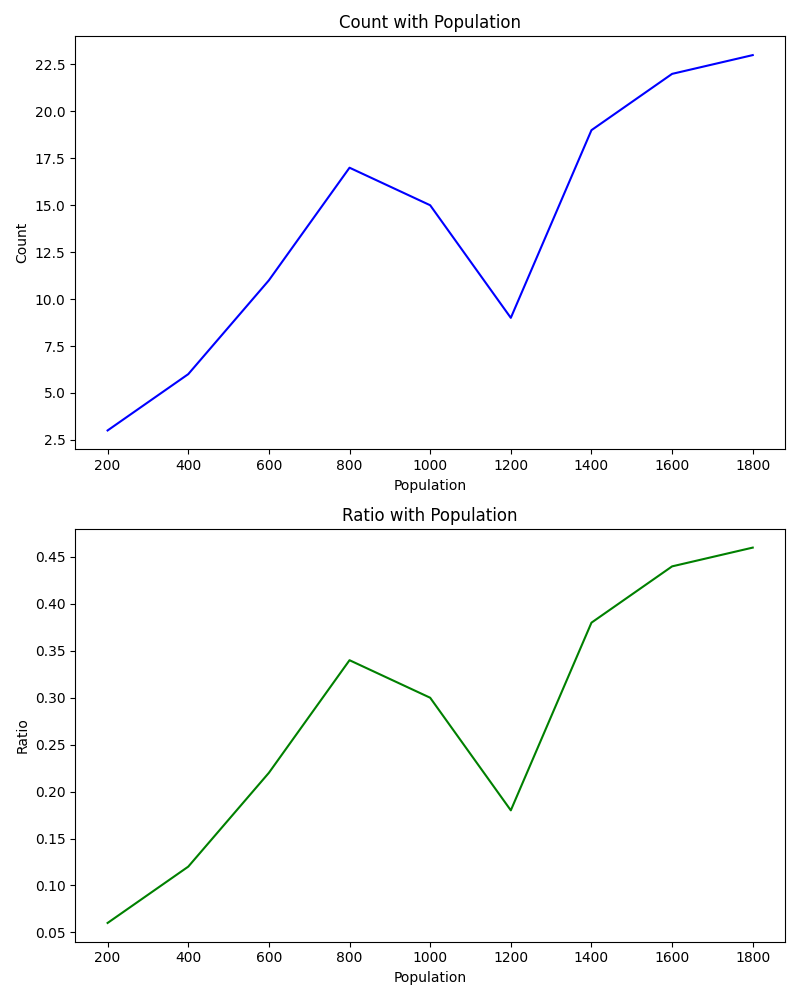
\includegraphics[scale = 0.5]{Figure_2.eps}
        \label{figure_2}
    \end{figure}

    \paragraph{6.结论:}
    古今中外有许多学者、数学家从不同的侧面作过生动的描述。古希腊数学家普洛克拉斯曾说:“哪里有数学,哪里就有美。
    ”英国大学者伯特兰·罗素更是用下面的文字形容他对数学之美的感受:“数学,如果正确地看它,则具有至高无上的美——正像雕刻的美,
    是一种冷而严肃的美,这种美不是投合我们天性的微弱的方面,这种美没有绘画或音乐的那些华丽的装饰,它可以纯净到崇高的地步,
    能够达到严格的只有最伟大的艺术才能显示的那种完美的境地。一种真实的喜悦的精神,一种精神上的亢奋,
    一种觉得高于人的意识——这些是至善至美的标准,能够在诗里得到,也能够在数学里得到。"这都是数学作为抽象的美,而Manderbrot-Set向我们展示的是
    数学的具象美,在强烈的视觉冲击下,无人不会不赞叹数学是多么奇妙的一门学科!
    \cite{Mandelbrot-Set-Summary}

\bibliographystyle{plain}
\bibliography{Forth}

\end{document}